\documentclass[12pt,a4paper,bibliography=totocnumbered,listof=totocnumbered]{article}
% u.U. muss Koma-Skript Package ueber MikTeX deinstalliert und neu installiert werden
% Hilft das nicht, so sollte statt scrartcl die Dokumentenklasse article verwendet werden
\usepackage[backend=bibtex,style=alphabetic]{biblatex}
\usepackage[ngerman,english]{babel}
\usepackage[utf8]{inputenc}
\usepackage{csquotes}
\usepackage{ifthen}
\usepackage{xargs}
\usepackage{amsmath}
\usepackage{amsfonts}
\usepackage{amssymb}
\usepackage{graphicx}
\usepackage{fancyhdr}
\usepackage{tabularx}
\usepackage{geometry}
\usepackage{multirow}
\usepackage{threeparttable}
\usepackage{xurl}
\usepackage{longtable}
\usepackage{makecell}
\usepackage{setspace}
\usepackage[right]{eurosym}
\usepackage[printonlyused]{acronym}
\usepackage{subfig}
\usepackage{floatflt}
\usepackage{float}
\usepackage[usenames,dvipsnames]{color}
\usepackage{colortbl}
\usepackage{paralist}
\usepackage{array}
\usepackage{parskip}
\usepackage[right]{eurosym}
\usepackage[subfigure,titles]{tocloft}
\usepackage[pdfpagelabels=true]{hyperref}
% added includes
\usepackage{tikz}
\usetikzlibrary{matrix,chains,positioning,decorations.pathreplacing,arrows}
\usepackage{pgfplots}
\usepackage{wrapfig}
\usepackage{listings}

\lstset{basicstyle=\footnotesize, captionpos=b, breaklines=true, showstringspaces=false, tabsize=2, frame=lines, numbers=left, numberstyle=\tiny, xleftmargin=2em, framexleftmargin=2em}
\makeatletter
\def\l@lstlisting#1#2{\@dottedtocline{1}{0em}{1em}{\hspace{1,5em} Lst. #1}{#2}}
\makeatother

\geometry{a4paper, top=27mm, left=20mm, right=20mm, bottom=35mm, headsep=10mm, footskip=12mm}

\definecolor{javared}{rgb}{0.6,0,0} % for strings
\definecolor{javagreen}{rgb}{0.25,0.5,0.35} % comments
\definecolor{javapurple}{rgb}{0.5,0,0.35} % keywords
\definecolor{javadocblue}{rgb}{0.25,0.35,0.75} % javadoc
\definecolor{gray}{rgb}{0.6,0.6,0.6}
 
\lstset{language=Java,
basicstyle=\ttfamily\footnotesize,
keywordstyle=\color{javapurple}\bfseries,
stringstyle=\color{javared},
commentstyle=\color{javagreen}\itshape\bfseries,
morecomment=[s][\color{javadocblue}]{/**}{*/},
numbers=left,
numberstyle=\tiny\color{gray},
stepnumber=1,
numbersep=10pt,
tabsize=3,
showspaces=false,
showstringspaces=false}
% Kopf- und Fusszeile
\renewcommand{\sectionmark}[1]{\markright{#1}}
\renewcommand{\leftmark}{\rightmark}
\pagestyle{fancy}
\lhead{}
\chead{}
\rhead{\thesection\space\contentsname}
\lfoot{}
\cfoot{}
\rfoot{\ \linebreak Page \thepage}
\renewcommand{\headrulewidth}{0.4pt}
\renewcommand{\footrulewidth}{0.4pt}

% Vorspann
\renewcommand{\thesection}{\Roman{section}}
\renewcommand{\theHsection}{\Roman{section}}
\pagenumbering{Roman}

\newcommand{\folgen}[1]{
\ensuremath
#1
}

\newcommandx{\student}[4][]{
	\def\studentName{#1}%
	\def\studentMatnr{#2}%
	\def\studentStudiengang{#3}%
	\def\studentEmail{#4}%
}

\newcommandx{\MyTitelseite}[8][]{
\thispagestyle{empty}

\includegraphics[scale=0.2]{pics/oth-logo.png}\hfill\includegraphics[scale=0.5]{#1}
\begin{center}
\ifthenelse{\equal{#2}{2}}{ % then
	\vspace*{2cm}
	\Large
	\textbf{Ostbayerische Technische Hochschule Regensburg}\\
	\textbf{University of Applied Sciences Regensburg}\\
	\textbf{Faculty of Computer Science and Mathematics}\\
	\vspace*{2cm}
	\Huge
	\textbf{#3}\\[1em]
	\large
	DevOps Principles and Practices\\
	\vspace*{1cm}
	\Large
	\textbf{#4}\\
}{ % else
	\vspace*{1cm}
	\Large
	\textbf{#4}\\
	\vspace*{2cm}
	\large
	Presented to the Faculty of Computer Science and Mathematics\\
	University of Applied Sciences Regensburg\\
	Study Subject: \\
	\studentStudiengang\\[2em]
	\vspace*{1cm}
	\Large
	\textbf{#3}\\[2em]
	\large
	In Partial Fulfillment of the Requirements for the Degree of\\
	\ifthenelse{\equal{#3}{Bachelor Thesis}}{Bachelor of Science (B.Sc.)}{Master of Science (M.Sc.)}
	\vspace*{1cm}
	\Large
}
	\vfill
	\normalsize
	\newcolumntype{x}[1]{>{\raggedleft\arraybackslash\hspace{0pt}}p{#1}}
	\begin{tabular}{rl}%{6cm}p{7.5cm}}
		\rule{0mm}{1ex}\textbf{Presented by:} & \studentName \\
		\rule{0mm}{1ex}\textbf{E-Mail:} & \studentEmail \\
		\rule{0mm}{1ex}\textbf{Student Number:} & \hspace*{-0.5em}\begin{tabular}[t]{r}\studentMatnr\end{tabular} \\ 
		\ifthenelse{\equal{#2}{1}}{~\\}{\rule{0mm}{1ex}\textbf{Study Subject:} & \studentStudiengang \\[2em]}
		\rule{0mm}{1ex}\textbf{Primary Supervising Professor:} & #5 \\ 
		\rule{0mm}{1ex}\textbf{Team:} & #6 \\[2em]
		\rule{0mm}{1ex}\textbf{Submission Date:} & #7 \\ 
	\end{tabular} 
\end{center}
\pagebreak
}
\addbibresource{literature.bib}

\begin{document}
\rule{\linewidth}{1pt}


% ----------------------------------------------------------------------------------------------------------
% Cover page
% ----------------------------------------------------------------------------------------------------------
\newcommand{\studierenderName}{Tianhua Dai}
\student{\studierenderName}		% Student's Name
{3111914}						% Student Number
{Business Informatics}			% Study Programme
{tianhua.dai@st.oth-regensburg.de}	% Student's Email

\MyTitelseite{pics/leer}	% Optionally Logo of Supervising Company
{2}								% Style of Cover Page (1 or 2)
{Assignment 1}				% Type of thesis (\in {Bachelor Thesis, Master Thesis})
{Tools for Version Control and Test Automation}				% Title of Thesis					
{Dr.\ Abhijit Sen}		% Primary Supervising Professor
{Jiawei Tang, Yue Yuan, Tianhua Dai}	% Team members
{22.05.2020}				% Submission Date

\thispagestyle{empty}
\pagebreak

%\setcounter{page}{1} 

% ----------------------------------------------------------------------------------------------------------
% Table of Contents
% ----------------------------------------------------------------------------------------------------------
\setcounter{tocdepth}{2}
\tableofcontents
\pagebreak

% ----------------------------------------------------------------------------------------------------------
% List of Figures
% ----------------------------------------------------------------------------------------------------------
\lhead{}
\rhead{List of Figures}
\listoffigures
\pagebreak

% ----------------------------------------------------------------------------------------------------------
% List of Tables (optional)
% ----------------------------------------------------------------------------------------------------------
\lhead{}
\rhead{List of Tables}
\listoftables
\pagebreak

% ----------------------------------------------------------------------------------------------------------
% Content
% ----------------------------------------------------------------------------------------------------------
% Spacing for Headlines

% Header
\renewcommand{\sectionmark}[1]{\markright{#1}}
\renewcommand{\subsectionmark}[1]{}
\renewcommand{\subsubsectionmark}[1]{}
\lhead{Chapter \thesection}
\rhead{\rightmark}

%\onehalfspacing
\setstretch{1.15}
\renewcommand{\thesection}{\arabic{section}}
\renewcommand{\theHsection}{\arabic{section}}
\setcounter{section}{0}
\pagenumbering{arabic}
\setcounter{page}{1}

% ----------------------------------------------------------------------------------
% Chapter: Introduction
% ----------------------------------------------------------------------------------
\section{Introduction}
DevOps is a concept of software culture, and there are different understandings and interpretations of the scope of this culture, especially automation practices. 
It aims to seamlessly extend Development to the Operation stage, break the barriers between the two in the traditional software process, simplify all aspects of the software life cycle, and promote the healthy, fast and continuous delivery of software.
\footnote[1]{\cite{ref1}, S. 5}  
\newline
The concept of DevOps was introduced as early as 2009. With the increasing development of new technologies and automation tools, it has been valued by enterprises in past years rapidly and started to be widely practiced. 
Research shows that the continuous, efficient and high-quality delivery of DevOps depends on the support of a high degree of automation tools, and automation is also the key to obtaining rapid feedback.
There are number and variety of tools for implementing DevOps functionalities, which involve multiple stages through software development. This assignment is aimed to research tools for Version Control and tools for Test Automation.
\newline
The structure of the remaining chapters of this assignment is organized as follows. The usage of selected two tools for version control would be introduced in chapter 2. 
And chapter 3 demonstrates the practices with selected tools for test automation. Each tool would be described in table form with specific features. After each description the implementations with examples would be explained using sample screenshots.
At last each tool would be concluded in a subsection.    
\newline
\pagebreak
% ----------------------------------------------------------------------------------
% Chapter: 
% ----------------------------------------------------------------------------------
\section{Tools for Version Control}
Version control is a system that records changes in the content of a file or set of files over time so that man can recall specific versions later.
The files that contain the software source code would be usually version-controlled, but in fact, version control is just for any file type, for example a thesis or report using Word.
\footnote[2]{\cite{ref2}}
Version control systems bring also some good benefits like compare files, identify differences, and merge the changes if needed. Another great use of versioning is keeping track during the whole software development process. 
\footnote[3]{\cite{ref3}}
Basically, the version control systems can differ in 3 types. (see table \ref{tab:VersionControlSystems})
\vspace{1em}
\begin{table}[!h]
	\centering
	\begin{tabular}{|l|l|l|}
		\hline
		\textbf{Typ} & \textbf{Representative product} & \textbf{Website} \\
		\hline
		Local & RCS & \url{https://gnu.org/software/rcs}\\
		\hline
		Centralized & SVN & \url{https://subversion.apache.org}\\
		\hline
		Distributed & Git & \url{https://git-scm.com} \\
		\hline
	\end{tabular}
	\caption{Version Control Systems}
	\label{tab:VersionControlSystems}
\end{table}
\newline
The local version control system is relatively simpler from a basic point of view, which has a simple database that keeps all the changes to files under revision control. 
In other words, the local type is now a basic functionality for version control. Systems from the other 2 types, such as Git and SVN, have realized many more functionalities when using specific tools.
So, the following contents of this chapter describe the usage of 2 representative tools, through which software release could be delivered faster and more efficiently. 
 
\subsection{GitHub}
\subsubsection{Introduction}
It is established that Git is a version control system. But what makes GitHub-A Tool for Version Control System-so special?
Because it is free and open-sourced. GitHub is a web interface for git repositories as well as a development platform for developers. It's built as a virtual community so that developers store their projects online and connect with other like-minded people.  
\footnote[4]{\cite{ref4}}  
Therefore, the following subsections demonstrate the description with some important attributes and then the performing by a sample.
\subsubsection{Description}
In this section the attributes of GitHub would be demonstrated in the following table. (see table \ref{tab:GitHub})
\vspace{1em}
\begin{table}[!h]
	\centering
	\begin{tabular}{|l|l|}
		\hline
		\textbf{Attribute} & \textbf{Contents} \\
		\hline
		Name & GitHub \\
		\hline
		Purpose & \makecell[l]{GitHub is a code sharing and publishing service \\ based on web platform. It is also a Git repository \\ hosting service, which provides the user-friendly GUI \\ and many its own features.} \\
		\hline
		Website & \url{https://github.com} \\
		\hline
		Version & - \\
		\hline
		Date & - \\
		\hline
		Features\footnotemark[5] & \makecell[l]{1. Support all functionalities by Git \\ 2. Access control and collaboration features \\ 3. Fork, pull request and merge} \\
		\hline
		Requirements/ Compatibility & Anyone browser \\
		\hline
		Cost & free \\
		\hline
	\end{tabular}
	\caption{GitHub description}
	\label{tab:GitHub}
\end{table}
\footnotetext[5]{\cite{ref5}}

\subsubsection{Sample}
My sample is a java project using features of TestNG and Selenium, which tests the login method in a web game.
This project has been published in GitHub repository (\url{https://github.com/Tianhua-Joseph-Dai/testAutomation_ddop}).
The following content could be divided into 3 parts in order to describe the practice using GitHub.
\begin{enumerate}
	\item Preparation: A new repository would be established in website at first. And then the link of this repository is available. (see figure \ref{fig:github01})
	\begin{figure}[H] 
		\begin{minipage}[t]{0.5\linewidth} 
		\centering 
		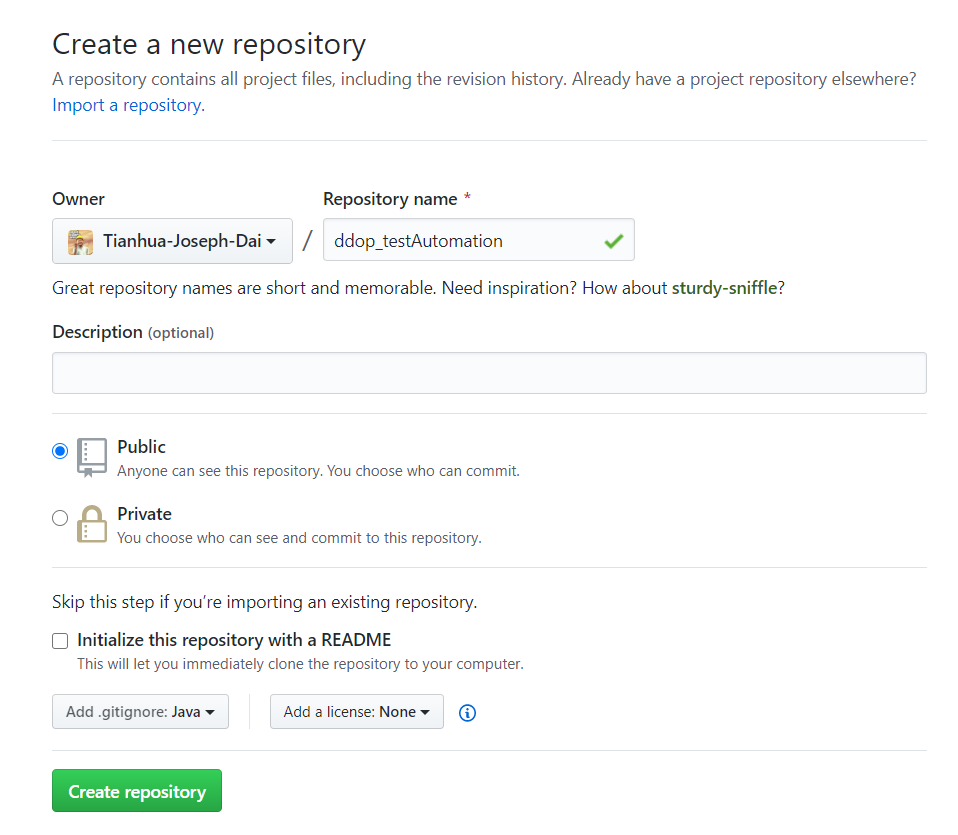
\includegraphics[width=2.5in]{pics/createNewOnline.png}  
		\end{minipage}% 
		\begin{minipage}[t]{0.5\linewidth} 
		\centering 
		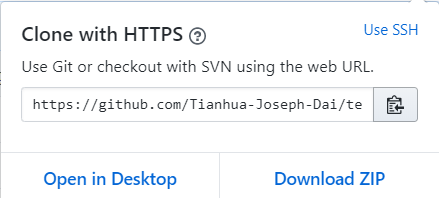
\includegraphics[width=2.5in]{pics/getUrl.png} 
		\end{minipage} %
		\caption{Create new repository and get the clone link}
		\label{fig:github01}
	\end{figure} %		
	\newpage
	At the same time a local folder has been prepared for cloning the remote project\\ by using Git Bash command. (see figure \ref{fig:github02})\\ 
	\begin{minipage}{\linewidth}
		\centering
		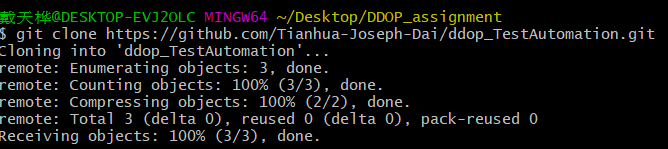
\includegraphics[width=0.5\linewidth]{pics/gitClone.png}
		\captionof{figure}[Pic Git Clone]{Clone into the local folder}
		\label{fig:github02}
	\end{minipage}
	\item Sample: Firstly, a new branch (test/openGoogle) was created in local, which matches the\\ functionality of program to add. The advantage of this operation is to consider version\\ control. After the add functionality and the commit with some infomation the project\\ would be pushed to the web platform in GitHub. (see figure \ref{fig:github03})
	\begin{figure}[H] 
		\begin{minipage}[t]{0.5\linewidth} 
		\centering 
		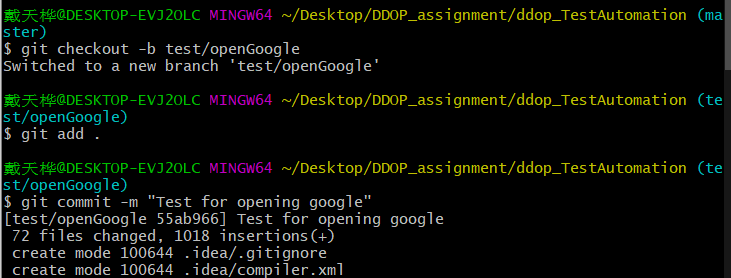
\includegraphics[width=2.5in]{pics/gitAdd.png}  
		\end{minipage}% 
		\begin{minipage}[t]{0.5\linewidth} 
		\centering 
		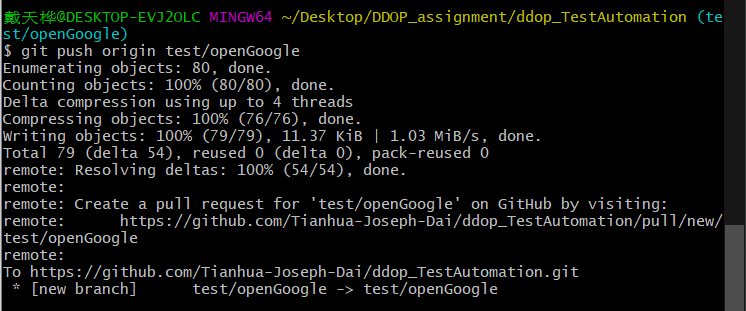
\includegraphics[width=2.5in]{pics/gitPush.png} 
		\end{minipage} %
		\caption{Commit the local changes and push them online}
		\label{fig:github03}
	\end{figure}
	At last the new branch would be also visible online in the repository. (see figure \ref{fig:github04})
	\newline
	\begin{minipage}{\linewidth}
		\centering
		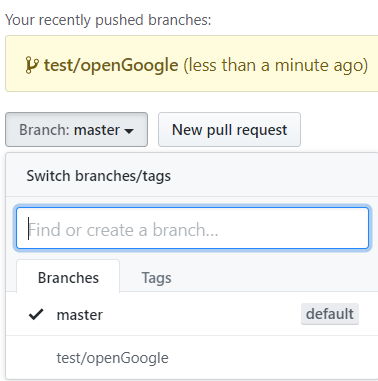
\includegraphics[width=0.5\linewidth]{pics/newBranchOnline.png}
		\captionof{figure}[Pic New Branch]{Update online}
		\label{fig:github04}
	\end{minipage}
	\item Maintenance: After any modification a new branch would be established as a new method\\
	in local repository. Therefore, the changes from other branches should be merged into master
	and make the whole project UpToDate. (see figure \ref{fig:github05})
	\begin{figure}[H] 
		\begin{minipage}[t]{0.5\linewidth} 
		\centering 
		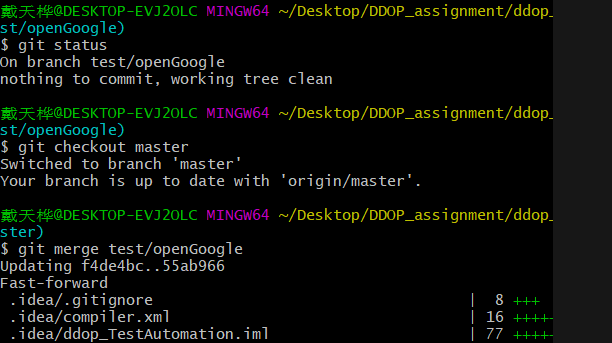
\includegraphics[width=2.5in]{pics/gitMerge.png}  
		\end{minipage}% 
		\begin{minipage}[t]{0.5\linewidth} 
		\centering 
		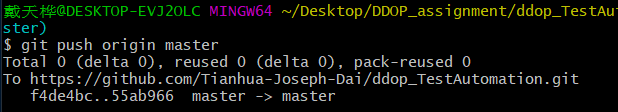
\includegraphics[width=2.5in]{pics/gitUpdate.png} 
		\end{minipage} %
		\caption{Merge the changes and update the project}
		\label{fig:github05}
	\end{figure}
\end{enumerate}

\subsection{Tortoise SVN}
\subsubsection{Introduction}
This section is about another type of version control system, which is different from Git.
Subversion is a centralized version control system, which now is developed as a project of the Apache Software Foundation. It has also been developing to a rich community for developers to widespread and collaborate.
\newline
Similar to Git SVN is also or just a command-line client. Tortoise SVN is built on the basis of SVN, which is performed as a windows shell extension. Tortoise SVN provides a easy user GUI for managing different versions of projects.

\subsubsection{Description}
The following table lists the attributes of Tortoise SVN. The content in the following table\\ is referenced from the Tortoise SVN website. (see table \ref{tab:TortoiseSVN})
\begin{table}[H]
	\centering
	\begin{longtable}{|l|l|}
		\hline
		\textbf{Attribute} & \textbf{Contents} \\
		\hline
		Name & Tortoise SVN \\
		\hline
		Purpose & \makecell[l]{Tortoise SVN is used for revision/version/source control.\\} \\
		\hline
		Website & \url{https://tortoisesvn.net} \\
		\hline
		Version & 1.13.1 \\
		\hline
		Date & 2019/11/01 \\
		\hline
		Features & \makecell[l]{1. Cover functionalities of SVN \\ 2. Support for all subversion protocols \\ 3. Integration with issue tracking systems\\ 4.Support from multiple language packs} \\
		\hline
		Requirements/ Compatibility & \makecell[l]{1. Windows 7 or later\\ 2. A SVN server} \\
		\hline
		Cost & free \\
		\hline
		Note & \makecell[l]{1. Tortoise SVN is not available for UNIX-OS yet.\\2. SVN server must be installed in advance.}\\
		\hline
	\end{longtable}
	\caption{Tortoise SVN description}
	\label{tab:TortoiseSVN}
\end{table}

\subsubsection{Sample}
The same project would be practiced in SVN system. It would be also divided into 3 parts to describe the implementation using Tortoise SVN.
\begin{enumerate}
	\item Preparation: Because Tortoise SVN is a SVN client, a SVN server is needed as requirement. VisualSVN Server (\url{https://visualsvn.vom/server}) is used to demonstrate in this sample. At first a new repository should be created. (see figure \ref{fig:svn01})
	\begin{figure}[H] 
		\begin{minipage}[t]{0.5\linewidth} 
		\centering 
		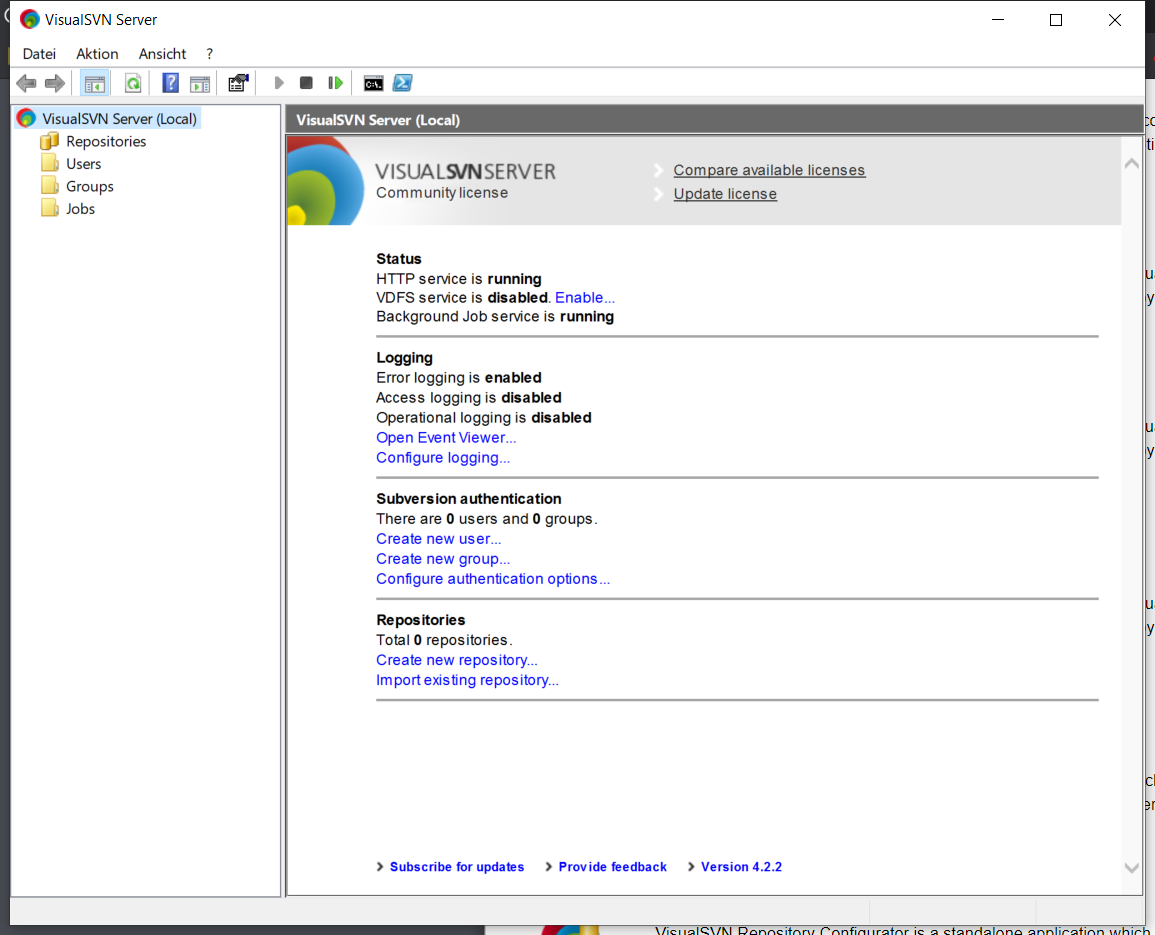
\includegraphics[width=2.5in]{pics/visualServer.png}  
		\end{minipage}% 
		\begin{minipage}[t]{0.5\linewidth} 
		\centering 
		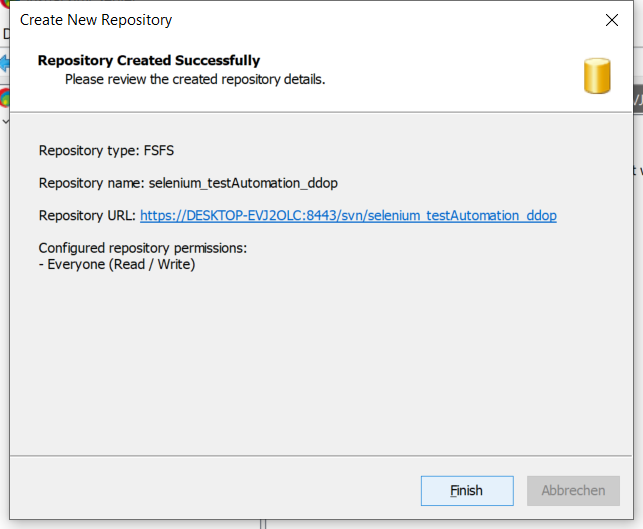
\includegraphics[width=2.5in]{pics/createSVNRepo.png} 
		\end{minipage} %
		\caption{Create new repository in VisualSVN}
		\label{fig:svn01}
	\end{figure} %
	Then open any windows explorer, right click, Tortoise SVN features are visible in the menu. Select the Repo-browser and enter the repository link. At last it succeed with access the repository. (see figure \ref{fig:svn02})
	\begin{figure}[H] 
		\begin{minipage}[t]{0.5\linewidth} 
		\centering 
		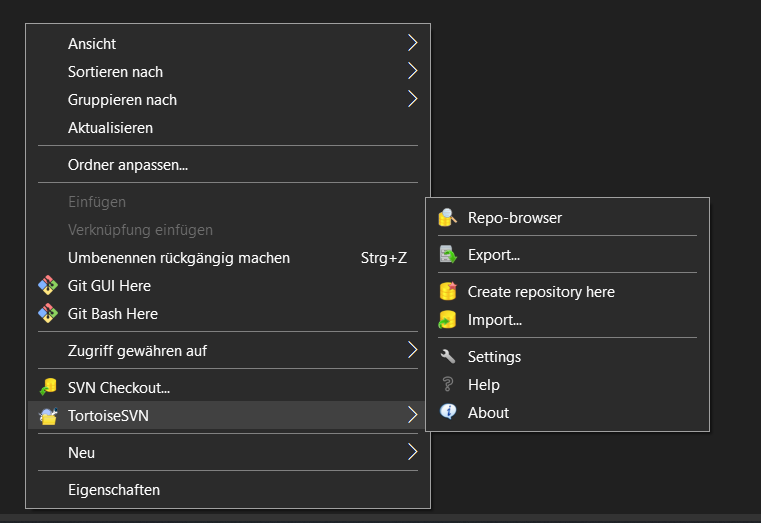
\includegraphics[width=2.5in]{pics/toSVNRepo.png}  
		\end{minipage}% 
		\begin{minipage}[t]{0.5\linewidth} 
		\centering 
		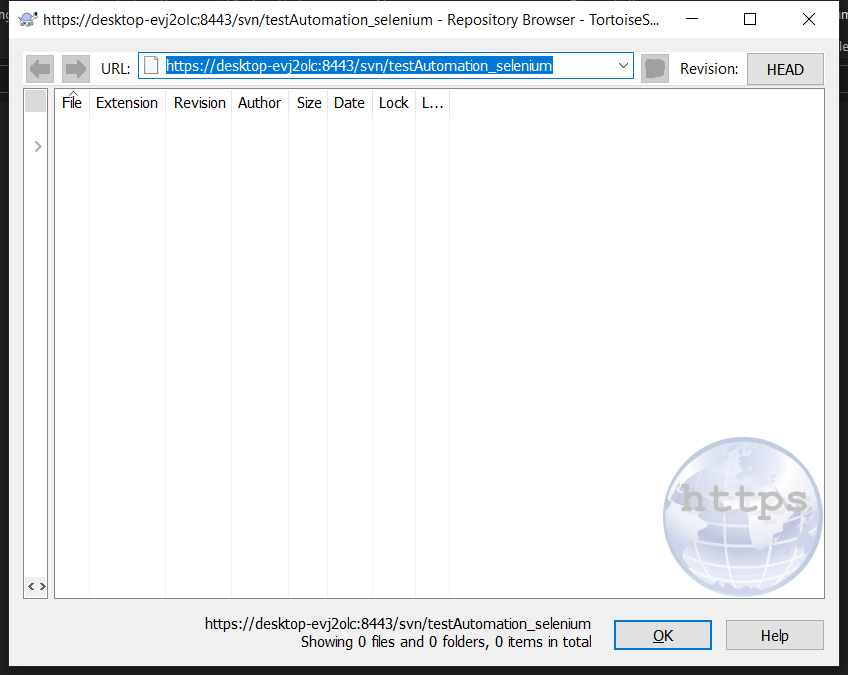
\includegraphics[width=2.5in]{pics/repoBrowser.png} 
		\end{minipage} %
		\caption{Link to repository using Tortoise SVN}
		\label{fig:svn02}
	\end{figure} %
	\item Sample: SVN has a relatively strict access control so that the user must firstly determine the authorities and set in the repository. After that the connect would be established by checkout, which is like the switch branch feature from Git. (see figure \ref{fig:svn03})
	\begin{figure}[H] 
		\begin{minipage}[t]{0.5\linewidth} 
		\centering 
		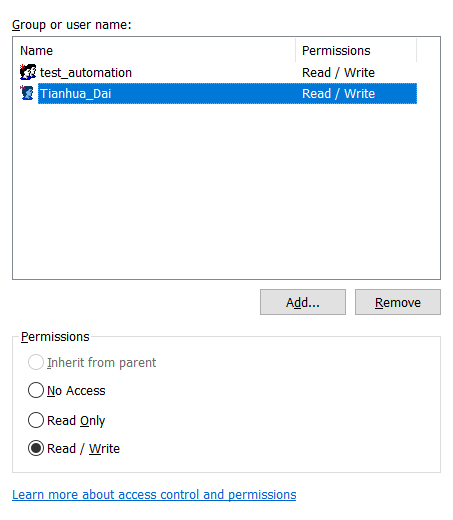
\includegraphics[width=2.5in]{pics/svnSetAuth.png}  
		\end{minipage}% 
		\begin{minipage}[t]{0.5\linewidth} 
		\centering 
		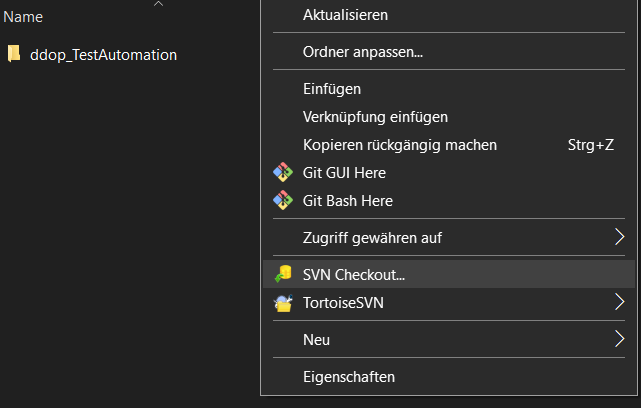
\includegraphics[width=2.5in]{pics/svnCheckout.png} 
		\end{minipage} %
		\caption{Set authorities and checkout}
		\label{fig:svn03}
	\end{figure} %
	User can right click in the local repository to commit the modification. The revision\\ number would be increased after a successful commit. At the same time the project\\ is also available in browser repository. (see figure \ref{fig:svn04})
	\vspace{1em}\\
	\begin{figure}[H] 
		\begin{minipage}[t]{0.5\linewidth} 
		\centering 
		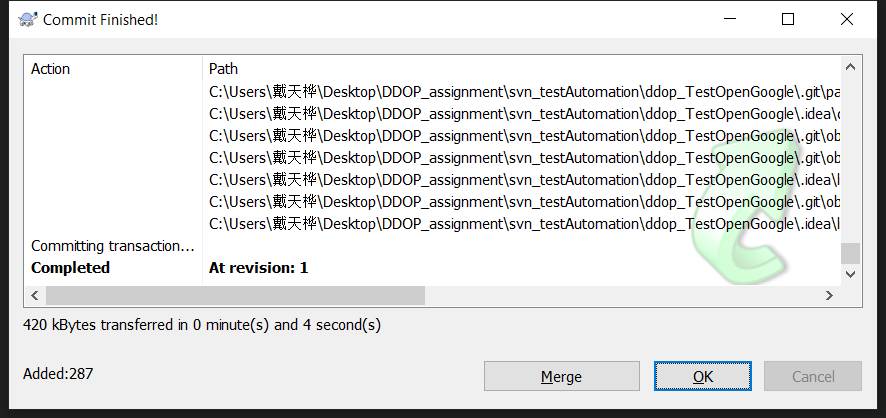
\includegraphics[width=2.5in]{pics/svnCommit.png}  
		\end{minipage}% 
		\begin{minipage}[t]{0.5\linewidth} 
		\centering 
		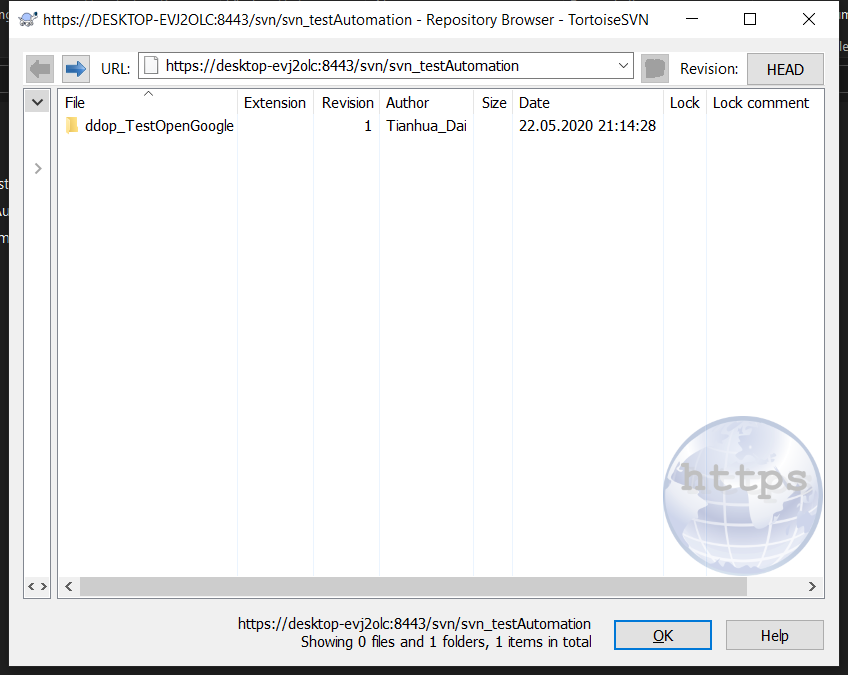
\includegraphics[width=2.5in]{pics/svnUpdate.png} 
		\end{minipage} %
		\caption{Commit with changes and update}
		\label{fig:svn04}
	\end{figure} %
	\item Maintenance: Furthermore, Tortoise SVN provides a log feature which support many useful functionalities to maintain the project. (see figure \ref{fig:svn05})
	\vspace{1em}\\
	\begin{minipage}{\linewidth}
		\centering
		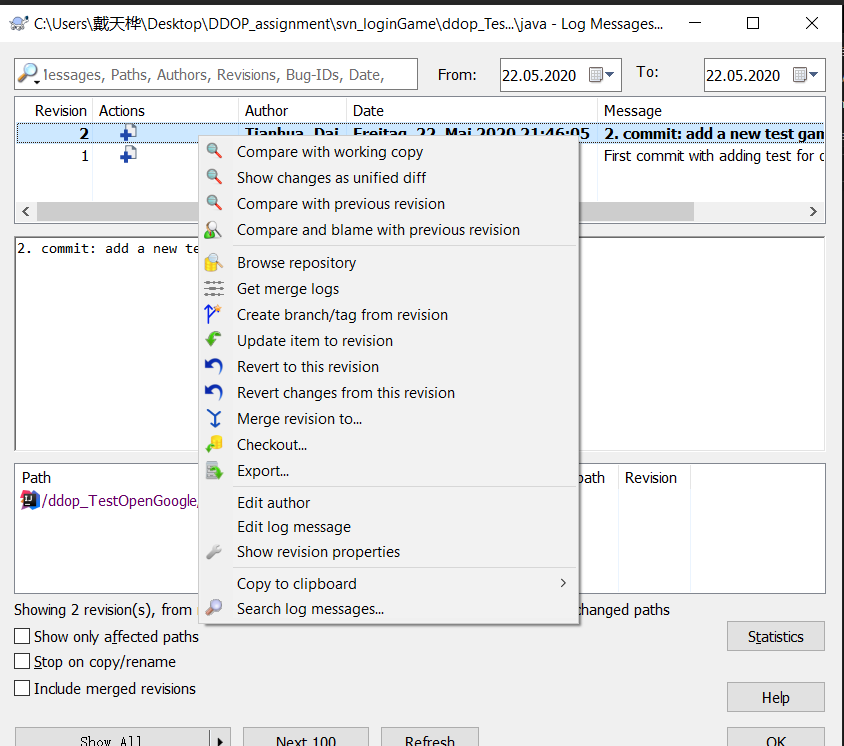
\includegraphics[width=0.5\linewidth]{pics/svnLog.png}
		\captionof{figure}[Pic SVN Log]{Log overview}
		\label{fig:svn05}
	\end{minipage}  
\end{enumerate} 

\subsection[Conclusion]{Conclusion\footnote[6]{\cite{ref6}}}
These tools support the implementation of the functions for version control systems in order to increase the work efficiency.
And with the continuous development the most functionalities of version control systems have been trending to one standard.
GitHub is a free, open-sourced web development platform for git repositories. It handles project versioning from some to very large projects efficiently and quickly.
The biggest difference between distributed and centralized is that, on the one hand developers can commit locally, 
and on the other hand each developer can copy a complete repository on their own PC through git cloning. Developers can also do their works without the internet. 
\newline
By contrast SVN manages data that changes over time. This data is kept in a central repository. So this archive could be seen as a normal file server, but it remembers
every changes. According to this restore to an old revision or browser through the history is allowed. Besides the core of centralized management is the server, 
where all developers must get code from the server at first. All version information is placed on the server. Without the server, developers basically can't work.

\pagebreak
% ----------------------------------------------------------------------------------
% Chapter: 
% ----------------------------------------------------------------------------------
\section{Tools for Test Automation}
\subsection{TestNG}
\subsubsection{Introduction}
TestNG is one of most popular testing frameworks, which inspired from JUnit and NUnit. It is designed to be competent for all kinds of testing cases.
In addition, TestNG is supported by a number of plugins and tools so that developers can make their test implementation easier and more efficient. 
\subsubsection{Description}
In this section the attributes of TestNG would be demonstrated in the following table (see table \ref{tab:TestNG}). The content is referenced from the official TestNG website.
\begin{table}[H]
	\centering
	\begin{tabular}{|l|l|}
		\hline
		\textbf{Attribute} & \textbf{Contents} \\
		\hline
		Name & TestNG \\
		\hline
		Purpose & \makecell[l]{TestNG is used for tests in unit, functional, integration etc..\\} \\
		\hline
		Website & \url{https://testng.org/doc} \\
		\hline
		Version & 7.1.0 \\
		\hline
		Date & 2019/12/27 \\
		\hline
		Features & \makecell[l]{1. Support almost all kinds of tests\\ 2. Test with multithread safety\\ 3. Supported by variety of plugins and tools} \\
		\hline
		Requirements/ Compatibility & JDK 7 or higher \\
		\hline
		Cost & free \\
		\hline
		Note & - \\
		\hline
	\end{tabular}
	\caption{TestNG description}
	\label{tab:TestNG}
\end{table}

\subsubsection{Sample}
A test can be easily built with the TestNG annotations, some test logics and configuration in a xml file. 
The sample to demonstrate is about login in a web game with different information. (see listing \ref{lst:loginTest})
\vspace{1em}
\lstinputlisting[caption=Login test, label=lst:loginTest,basicstyle=\ttfamily\scriptsize]{code/codeGameLogin.txt}
The selenium framework supports the necessary web functionalities in this program.\\ And this test will run in several cases (test cases \ref{fig:login01}) through data provider.\\ 
(Result of implementation )
\newline
	\begin{figure}[H] 
		\begin{minipage}[t]{0.5\linewidth} 
		\centering 
		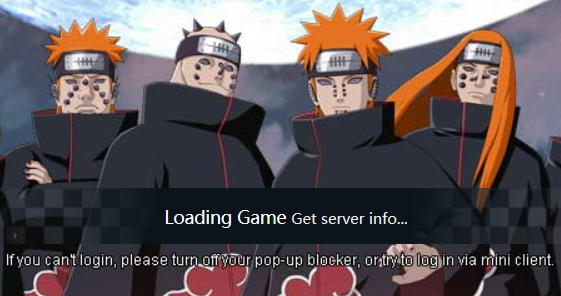
\includegraphics[width=2.5in]{pics/login01.png}  
		\end{minipage}% 
		\begin{minipage}[t]{0.5\linewidth} 
		\centering 
		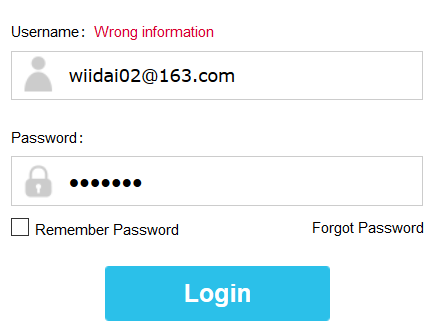
\includegraphics[width=2.5in]{pics/login02.png} 
		\end{minipage} %
		\begin{minipage}[t]{0.5\linewidth} 
		\centering 
		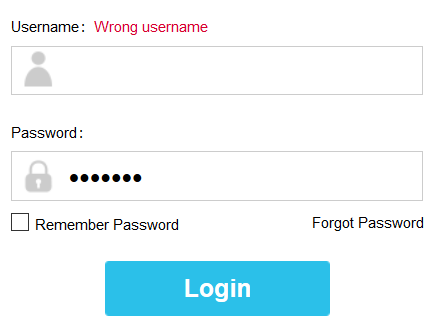
\includegraphics[width=2.5in]{pics/login03.png} 
		\end{minipage} %
		\begin{minipage}[t]{0.5\linewidth} 
		\centering 
		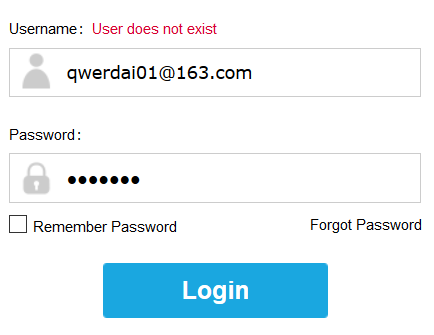
\includegraphics[width=2.5in]{pics/login04.png} 
		\end{minipage} %
		\caption{Different test cases}
		\label{fig:login01}
	\end{figure} %
	\begin{minipage}{\linewidth}
		\centering
		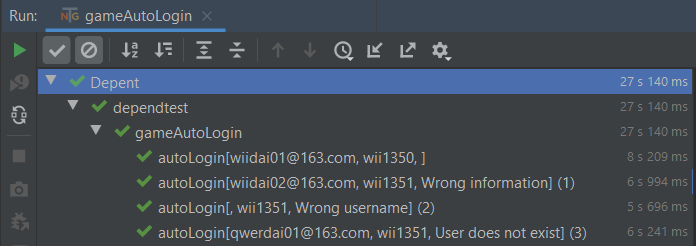
\includegraphics[width=0.5\linewidth]{pics/login05.png}
		\captionof{figure}[Pic Test Result]{Result of test}
		\label{fig:login02}
	\end{minipage} 

\subsection{SoapUI}
\subsubsection{Introduction}
SoapUI is an open source testing tool, which covers a variety of tests for web services. 
It has an easy-to-use graphical interface and supports all standards of protocols and technologies of web.
\subsubsection{Description}
The attributes of SoapUI would be demonstrated in the following table. The following content is referenced from the official SoapUI website.
\begin{table}[H]
	\centering
	\begin{tabular}{|l|l|l|l|}
	\hline
	Attribute                                                          & \multicolumn{3}{l|}{Contents}                           \\ \hline
	Name                                                               & \multicolumn{3}{l|}{SoapUI}                             \\ \hline
	Purpose                                                            & \multicolumn{3}{l|}{\makecell[l]{SoapUI is used for web services testing for SOA and REST. \\ Main functionalities cover exploring, mocking, load, \\ functional and security testing for web services.}}  \\ \hline
	Website                                                            & \multicolumn{3}{l|}{\url{https://www.soapui.org}}        \\ \hline
	Version                                                            & \multicolumn{3}{l|}{5.5.0}                                   \\ \hline
	Date                                                               & \multicolumn{3}{l|}{2019/02/12}                                   \\ \hline
	Features                                              			   & \multicolumn{3}{l|}{\makecell[l]{1. Multiple web service tests \\ 2. Web services mocking and inspection \\ 3. Data-driven tests and test automation \\ 4. API monitoring, HTTP recording}}                                   \\ \hline
	\multicolumn{1}{|c|}{\multirow{2}{*}{Requirements/ Compatibility}} & Windows                     & \multicolumn{2}{l|}{\makecell{Windows XP or later \\ Java 7}}     \\ \cline{2-4} 
	\multicolumn{1}{|c|}{}                                             & UNIX                        & \multicolumn{2}{l|}{\makecell{Ubuntu, Red Hat, Fedora, etc. \\ Java 7}}     \\ \hline
	\multirow{3}{*}{Cost}                                              & SoapUI Open Source          & \multicolumn{2}{l|}{free} \\ \cline{2-4} 
																	   & \multirow{2}{*}{SoapUI Pro} & Fixed License       &	€640/year     \\ \cline{3-4} 
																	   &                             & Floating License    &	€4,100/year     \\ \hline
	Notes                                                              & \multicolumn{3}{l|}{-}                                   \\ \hline
	\end{tabular}
	\caption{SoapUI description}
	\label{tab:SoapUI}
\end{table} %

\subsubsection{Sample}
The sample to practice is a test with several steps, which finally get the TV program information from a certain channel on a set date.
At first a SOAP or REST project would be created by inputted URL. Then run the requests to find out the parameters which are necessary for the test suite.
After several processes a test suite with the test case was generated, that to search TV program from Shanghai East TV Channel. (see figure \ref{fig:soap01}) 
\begin{figure}[H] 
	\begin{minipage}[t]{0.5\linewidth} 
	\centering 
	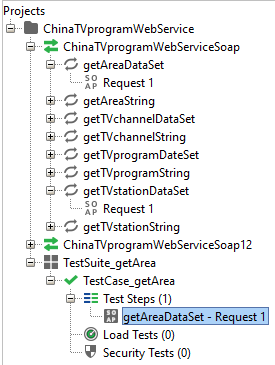
\includegraphics[width=2.5in]{pics/soap01.png}
	\end{minipage}% 
	\begin{minipage}[t]{0.5\linewidth} 
	\centering 
	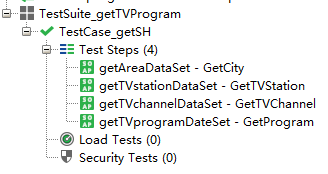
\includegraphics[width=2.5in]{pics/soap02.png} 
	\end{minipage} %
	\caption{Create a completed test case}
	\label{fig:soap01}
\end{figure}
Then the xml file of each request must be added by parameter. (see listing \ref{lst:soapParam})
\vspace{1em}
\lstinputlisting[caption=Request with parameter, label=lst:soapParam,basicstyle=\ttfamily\scriptsize]{code/codeSOAPParam.txt}
Furthermore a important step is to generate a assertion to each request. Through the assertion the result could be detected easier. (see figure \ref{fig:soap02})
\begin{figure}[H] 
	\begin{minipage}[t]{0.5\linewidth} 
	\centering 
	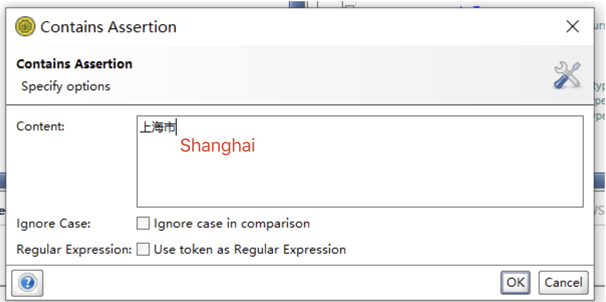
\includegraphics[width=2.5in]{pics/soap03.png}
	\end{minipage}% 
	\begin{minipage}[t]{0.5\linewidth} 
	\centering 
	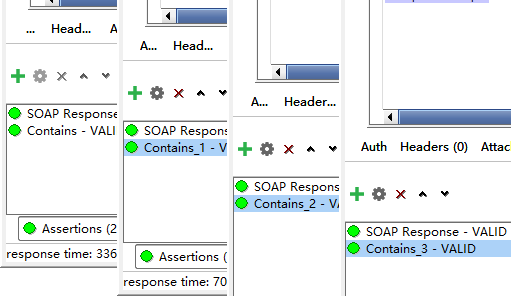
\includegraphics[width=2.5in]{pics/soap04.png} 
	\end{minipage} %
	\caption{Set the assertion and results}
	\label{fig:soap02}
\end{figure}

\subsection{Conclusion}
It is established that web services are called by programs, which generally do not provide interfaces for end user or tester directly.
Underlying, call relationships as well as protocols should be taken into consideration. SoapUI is a such a tool
so that user can complete tests in SoapUI with simple operations while it reduces workload. On the other hand TestNG provides
developers multiple test functions while they are developing. The program could be tested for different purposes. On the one hand it is supported by variety of plugins and tools,
on the other hand TestNG will be integrated in different projects as well. It could be a good element for a DevOps toolchain.

\pagebreak

% ----------------------------------------------------------------------------------------------------------
% Filter fuer Literatur und Quellen definieren
% ----------------------------------------------------------------------------------------------------------

%\defbibheading{Literatur}{\section*{Literaturverzeichnis}} 
\defbibheading{Quellen}{\section*{List of References}} 
  
%\defbibfilter{Literatur}{\not\keyword{online}} 
\defbibfilter{Quellen}{\keyword{online}}

% ---------------------------------------------------------------------------------------------------------- 
% Quellen 
% ---------------------------------------------------------------------------------------------------------- 
\lhead{} 
\rhead{Quellenverzeichnis} 

\printbibliography[title = {Quellenverzeichnis}, heading=Quellen,filter=Quellen]


\pagebreak

\end{document}
